\begin{center}
    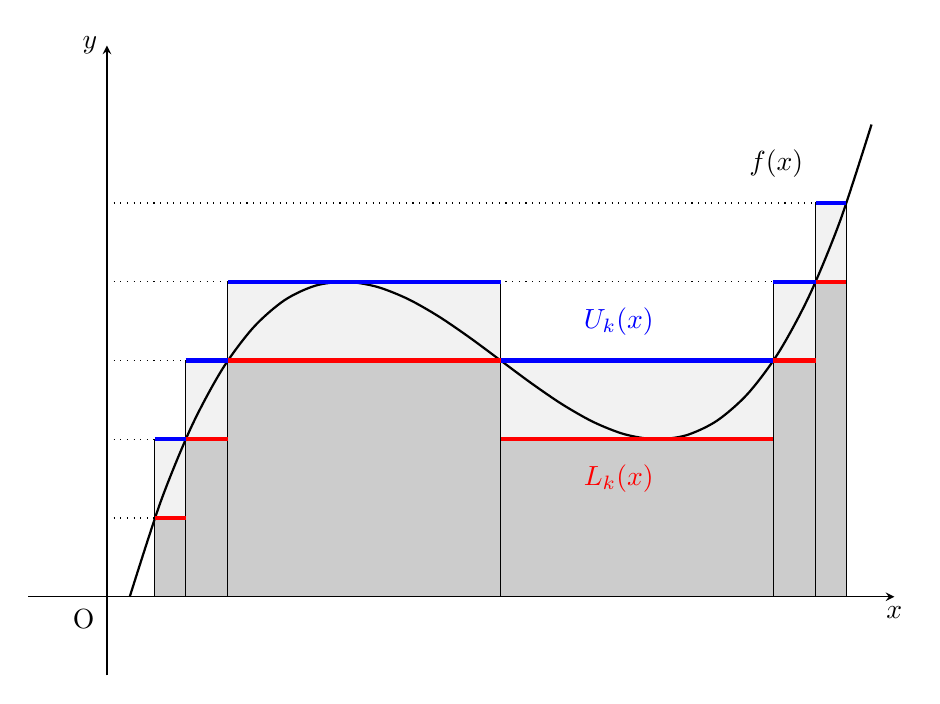
\begin{tikzpicture}[
            Lk/.style={red, ultra thick},
            Uk/.style={blue, ultra thick},
            dots/.style={thin, dotted},
            lower/.style={fill=gray!40, draw=black},
            upper/.style={fill=gray!10, draw=black},
        ]
        \node[below left=1pt] (origin) at (0,0) {\(\rm{O}\)};
        \draw [-stealth] (-1, 0) -- (10, 0) node[below] {\(x\)};
        \draw [-stealth] (0, -1) -- (0, 7) node[left] {\(y\)};

        \draw[dots] (0, 1) -- (0.6083, 1);
        \draw[dots] (0, 2) -- (1, 2);
        \draw[dots] (0, 3) -- (8.4641, 3);
        \draw[dots] (0, 4) -- (9.3916, 4);
        \draw[dots] (0, 5) -- (9.3916, 5);

        \pgfmathsetmacro{\maxn}{3}
        \pgfmathsetmacro{\limit}{24}

        \filldraw[upper] (0.6083, 2) rectangle (1, 0);
        \filldraw[upper] (1, 3) rectangle (1.5358, 0);
        \filldraw[upper] (1.5358, 4) rectangle (5, 0);
        \filldraw[upper] (5, 3) rectangle (8.4641, 0);
        \filldraw[upper] (8.4641, 4) rectangle (9, 0);
        \filldraw[upper] (9, 5) rectangle (9.3916, 0);

        \filldraw[lower] (0.6083, 1) rectangle (1, 0);
        \filldraw[lower] (1, 2) rectangle (1.5358, 0);
        \filldraw[lower] (1.5358, 3) rectangle (5, 0);
        \filldraw[lower] (5, 2) rectangle (8.4641, 0);
        \filldraw[lower] (8.4641, 3) rectangle (9, 0);
        \filldraw[lower] (9, 4) rectangle (9.3916, 0);

        \draw[thick,domain=0.2893:9.71, smooth, variable=\x] plot ({\x}, {-3.0625 + 3.9375*\x - 0.9375*\x^2 + \x^3/16 + 2});

        \draw[Lk] (0.6083, 1) -- (1, 1);
        \draw[Lk] (1, 2) -- (1.5358, 2);
        \draw[Lk] (1.5358, 3) -- (5, 3);
        \draw[Lk] (5, 2) -- (8.4641, 2);
        \draw[Lk] (8.4641, 3) -- (9, 3);
        \draw[Lk] (9, 4) -- (9.3916, 4);

        \draw[Uk] (0.6083, 2) -- (1, 2);
        \draw[Uk] (1, 3) -- (1.5358, 3);
        \draw[Uk] (1.5358, 4) -- (5, 4);
        \draw[Uk] (5, 3) -- (8.4641, 3);
        \draw[Uk] (8.4641, 4) -- (9, 4);
        \draw[Uk] (9, 5) -- (9.3916, 5);

        \node at (8.5, 5.5) {\(f(x)\)};
        \node[blue] at (6.5, 3.5) {\(U_k(x)\)};
        \node[red] at (6.5, 1.5) {\(L_k(x)\)};
    \end{tikzpicture}
\end{center}

\section*{Comparison with the Riemann Integral}

먼저 혼동을 막기 위해 Lebesgue measure \(m\)에 대하여 르벡 적분을
\[
    \int_{[a, b]} f \d{m} = \int_{[a, b]} f \d{x} = \int_a^b f \d{x}
\]
와 같이 표기하고, 리만 적분은
\[
    \mc{R}\int_a^b f\d{x}
\]
로 표기하겠습니다.

\thm{11.33} \(a, b \in \R\) 에 대하여 \(a < b\) 이고 함수 \(f\)가 유계라고 하자.
\begin{enumerate}
    \item \(f \in \mc{R}[a, b]\) 이면 \(f \in \mc{L}^{1}[a, b]\) 이고 \(\ds \int_a^b f\d{x} = \mc{R}\int_a^b f \d{x}\) 이다.
    \item \(f \in \mc{R}[a, b]\) \(\iff\) \(f\)가 연속 \(m\)-\ae on \([a, b]\).
\end{enumerate}

쉽게 풀어서 적어보면, (1)은 \(f\)가 \([a, b]\)에서 리만 적분 가능하면 르벡 적분 또한 가능하며, 적분 값이 같다는 의미입니다. 즉 르벡 적분이 리만 적분보다 더 강력하다는 것을 알 수 있습니다.

또한 (2)는 리만 적분 가능성에 대한 동치 조건을 알려줍니다. Almost everywhere라는 조건이 붙었기 때문에, \(\mc{L}^1\)의 equivalence class를 고려하면 사실상 연속함수에 대해서만 리만 적분이 가능하다는 뜻이 됩니다.

\pf \(k \in \N\) 에 대하여 구간 \([a, b]\)의 분할 \(P_k = \{a = x_0^k < x_1^k < \cdots < x_{n_k}^k = b\}\) 를 잡는다. 단 \(P_k \subset P_{k+1}\) (refinement) 이고 \(\abs{x_{i}^k - x_{i-1}^k} < \frac{1}{k}\) 이 되도록 한다.

그러면 리만 적분의 정의로부터
\[
    \lim_{k \ra \infty} L(P_k, f) = \mc{R}\lint{a}{b} f\d{x}, \quad \lim_{k \ra \infty} U(P_k, f) = \mc{R} \uint{a}{b} f \d{x}
\]
임을 알 수 있다.

이제 measurable simple function \(U_k, L_k\)를 다음과 같이 잡는다.
\[
    U_k = \sum_{i=1}^{n_k} \sup_{x_{i-1}^k \leq y \leq x_{i}^k} f(y) \chi_{(x_{i-1}^k, x_i^k]}, \quad L_k = \sum_{i=1}^{n_k} \inf_{x_{i-1}^k \leq y \leq x_{i}^k} f(y) \chi_{(x_{i-1}^k, x_i^k]}.
\]
그러면 구간 \([a, b]\) 위에서 \(L_k \leq f \leq U_k\)인 것은 당연하고, 르벡 적분이 가능하므로
\[
    \int_a^b L_k \d{x} = L(P_k, f), \quad \int_a^b U_k \d{x} = U(P_k, f)
\]
이 됨을 알 수 있다. 여기서 \(P_k \subset P_{k + 1}\) 이 되도록 잡았기 때문에, \(L_k\)는 증가하는 수열, \(U_k\)는 감소하는 수열이다.

그러므로
\[
    L(x) = \lim_{k \ra \infty} L_k(x), \quad U(x) = \lim_{k \ra \infty} U_k(x)
\]
로 정의했을 때, 극한이 존재함을 알 수 있다. 여기서 \(f, L_k, U_k\)가 모두 유계인 함수이므로 지배 수렴 정리에 의해
\[
    \int_a^b L \d{x} = \lim_{k \ra \infty} \int_a^b L_k \d{x} = \lim_{k \ra\infty} L(P_k, f) = \mc{R}\lint{a}{b} f\d{x} < \infty,
\]
\[
    \int_a^b U\d{x} = \lim_{k \ra \infty} \int_a^b U_k \d{x} = \lim_{k \ra\infty} U(P_k, f) = \mc{R} \uint{a}{b} f \d{x} < \infty
\]
이므로 \(L, U \in \mc{L}^{1}[a, b]\) 이다.

위 사실을 종합하면 \(f \in \mc{R}[a, b]\) 일 때,
\[
    \mc{R}\lint{a}{b} f\d{x} = \mc{R}\uint{a}{b} f\d{x}
\]
이므로
\[
    \int_a^b (U - L)\d{x} = 0
\]
가 되어 \(U = L\) \(m\)-\ae on \([a, b]\)라는 사실을 알 수 있다. 역으로 이를 거꾸로 읽어보면 \(U = L\) \(m\)-\ae on \([a, b]\)일 때 \(f \in \mc{R}[a, b]\) 가 되는 것 또한 알 수 있다.

\note{1} 위 논의에 의해 \(f \in \mc{R}[a, b]\) 이면 \(f = U = L\) \ae on \([a, b]\) 이다. 따라서 \(f\)는 measurable.
\[
    \int_a^b f \d{x} = \mc{R}\int_a^b f\d{x} < \infty \implies f \in \mc{L}^{1}[a, b].
\]

\note{2} 만약 \(x \notin \bigcup_{k=1}^{\infty} P_k\) 라고 가정하면, 임의의 \(\epsilon > 0\) 에 대해 충분히 큰 \(n \in \N\) 을 잡았을 때 적당한 \(j_0 \in \N\) 이 존재하여 \(x \in (t_{j_0-1}^n, t_{j_0}^n)\) 이면서
\[
    \abs{L_n(x) - L(x)} + \abs{U_n(x) - U(x)} < \epsilon
\]
이 되도록 할 수 있다. 그러면 \(y \in (t_{j_0-1}^n, t_{j_0}^n)\) 일 때
\[
    \begin{aligned}
        \abs{f(x) - f(y)} & \leq M_{j_0}^n - m_{j_0}^n = M_{j_0}^n - U(x) + U(x) - L(x) + L(x) - m_{j_0}^n \\
                          & \leq U(x) - L(x) + \epsilon
    \end{aligned}
\]
가 됨을 알 수 있다.

위 부등식에 의해 \(y \in \{x : U(x) = L(x)\} \bs \bigcup_{k=1}^{\infty} P_k\) 이면 \(f\)가 \(y\)에서 연속임을 알 수 있게 된다.

따라서, \(f\)가 연속인 점들의 집합을 \(C_f\)라 하면
\[
    \{x : U(x) = L(x)\} \bs \bigcup_{k=1}^{\infty} P_k \subset C_f \subset \{x : U(x) = L(x)\}
\]
이 된다. 한편 \(\bigcup_{k=1}^{\infty} P_k\)는 measure가 0 이므로, \(U = L\) \(m\)-\ae 인 것과 \(f\)가 연속 \(m\)-\ae 인 것은 동치이다. 위 논의의 결과를 이용하면 \(f \in \mc{R}[a, b]\) 인 것과 \(f\)가 연속 \(m\)-\ae 인 것은 동치이다.

아래는 증명의 부산물입니다.

\rmk
\begin{enumerate}
    \item \(x \notin \bigcup_{k=1}^\infty P_k\) 이면 \(f\)가 \(x\)에서 연속 \(\iff f(x) = U(x) = L(x)\) 이다.
    \item \(L(x) \leq f(x) \leq U(x)\) 이고 measurable function의 극한인 \(L(x), U(x)\) 또한 measurable이다.
    \item \(f\)가 유계라는 조건이 있기 때문에 \(f \geq 0\) 인 경우만 생각해도 충분하다. \(\abs{f} \leq M\) 라고 하면 \(f\) 대신 \(f + M\) 을 생각하면 되기 때문이다.
\end{enumerate}

이제 리만 적분의 유용한 성질들을 가지고 와서 사용할 수 있습니다.

\begin{enumerate}
    \item \(f \geq 0\) 이고 measurable일 때, \(f_n = f\chi_{[0, n]}\)으로 정의한다. 단조 수렴 정리에 의해
          \[
              \int_0^\infty f \d{x} = \lim_{n \ra \infty} \int_0^\infty f_n \d{x} = \lim_{n \ra \infty} \int_0^n f \d{x}
          \]
          이다. 마지막 적분을 리만 적분으로 계산할 수 있다.

    \item 닫힌 유계 구간 \(I \subset (0, \infty)\) 에 대하여 \(f \in \mc{R}(I)\) 라 하면 \(f \in \mc{L}^{1}(I)\) 이다. \(f_n = f\chi_{[0, n]}\) 으로 잡으면 \(\abs{f_n} \leq f\) 이므로 지배 수렴 정리를 적용하여
          \[
              \int_0^\infty f \d{x} = \lim_{n \ra \infty} \int_0^\infty f_n \d{x} = \lim_{n \ra \infty} \int_0^n f \d{x} = \lim_{n \ra \infty} \mc{R} \int_0^n f \d{x}
          \]
          임을 알 수 있다.

          마찬가지로 \(f_n = f\chi_{(1/n, 1)}\) 으로 잡은 경우에도 지배 수렴 정리에 의해
          \[
              \int_0^1 f\d{x} = \lim_{n \ra \infty} \int_{0}^1 f_n \d{x} = \lim_{n \ra \infty}\int_{1/n}^1 f \d{x} = \lim_{n \ra \infty} \mc{R}\int_{1/n}^1 f \d{x}
          \]
          이 된다.
\end{enumerate}

\pagebreak
